\section{Konstruktion des Aufbaus}

Für ein ressourcenschonendes Arbeiten ist es von großer Bedeutung neben den Methoden der Produktentwicklung auch diejenigen Materialien zu verwenden, die ohnehin schon vorrätig sind. In den entsprechenden Abschnitten wird noch näher drauf eingegangen. Zu bemerken sei aber noch, dass eine Verwendung der verfügbaren Materialien nicht immer die beste Option ist.

\subsection{Basisstativ}

In dem Labor \glqq Urban Mobility Lab\grqq\ liegt bereits das Fotostativ Manfrotto 055 bereit und kann verwendet werden. Herausfordernd kommt aber hinzu, dass sich ein 1/4\grqq\ Gewinde auf der Montageplatte befindet. Die folgenden Möglichkeiten zum Umgang mit dem Gewinde wurden diskutiert:

\begin{itemize}
	\item Nutenstein mit 1/4\grqq\ Innengewinde
	\item Adapterplatte zwischen Montageplatte und Trägerprofil
	\item Tausch der 1/4\grqq\ Schraube durch eine Schraube mit M4 Außengewinde
	\item Tausch des Stativs
\end{itemize}

Nach einer Anfrage bei der Firma \glqq item Industrietechnik GmbH\grqq\ nach Nutensteinen mit entsprechendem 1/4\grqq\ Innengewinde, war bekannt, dass sich derartige Produkte auf dem Markt nicht ohne Weiteres besorgen lassen.

Der Tausch des Stativs durch ein alternatives, ebenfalls zur Verfügung stehendes, wurde ausgeschlossen, da die Dimensionen des Stativs eindeutig zu massiv sind und der Anforderung einer leichten Transportierbarkeit im Wege stehen.

Eine Adapterplatte aus einem Aluminium-Flachprofil wurde ausgeschlossen, da nach einer Untersuchung des Fotostativs sich herauskristallisiert hat, dass die eingebaute UNC Schraube einfach durch eine M4 Schraube getauscht werden kann.

\subsection{Mikrofongehäuse}

Dadurch, dass die zum Einsatz kommenden Mikrofone fertig auf einer Platine (\autoref{fig:Mikrofonplatine}) verbaut sind, aber damit nicht gegen Regenwasser geschützt sind, mussten im Entwicklungsprozess Gehäuse für die Mikrofone konstruiert und 3D-gedruckt werden. Nach sehr kurzer Diskussion war beschlossen, dass mittels CAD-Technologie Gehäuse konstruiert und sie mit dem im Labor vorhandenen 3D-Drucker gefertigt werden sollen (\autoref{fig:Mikrofongehäuse}).

\begin{figure}[h]
	\begin{center}
		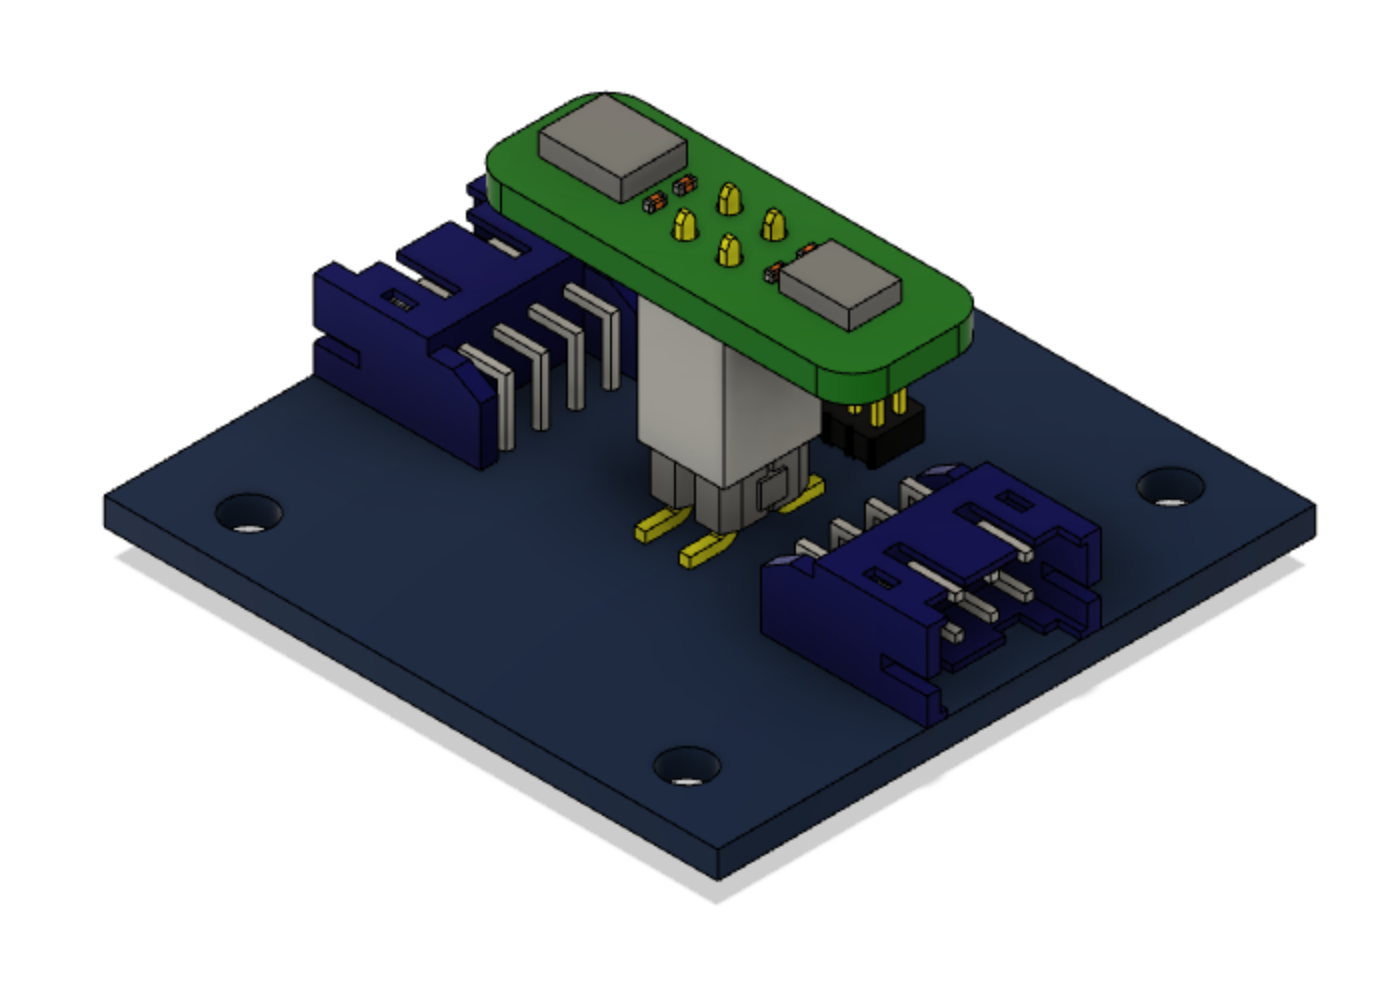
\includegraphics[scale=0.25]{Sections/Konstruktion_des_Aufbaus/Mikrofonplatine}
	\end{center}
	\caption{Mikrofonplatine}
	\label{fig:Mikrofonplatine}
\end{figure}

\newpage

\begin{figure}[h]
	\begin{center}
		\includegraphics[scale=0.25]{Sections/Konstruktion_des_Aufbaus/Mikrofongehäuse}
	\end{center}
	\caption{Mikrofongehäuse}
	\label{fig:Mikrofongehäuse}
\end{figure}

In der ersten Version dieser Gehäuse (\autoref{fig:Mikrofongehäuse_V_0.1}) soll die Mikrofonplatine über Stifte an Position gehalten und der Gehäusedeckel im Anschluss durch einen Längspressverband mit dem Gehäuseboden verbunden werden.

\begin{figure}[h]
	\begin{center}
		\includegraphics[scale=0.2]{Sections/Konstruktion_des_Aufbaus/Mikrofongehäuse_V_0.1}
	\end{center}
	\caption{Mikrofongehäuse V 0.1}
	\label{fig:Mikrofongehäuse_V_0.1}
\end{figure}


Nach dem Druck der sechs Gehäuse stellte sich heraus, dass:

\begin{enumerate}
	\item die gedruckten Stifte nicht maßhaltig sind
	\item die Löcher im Deckel nicht maßhaltig sind
	\item viele druckbedingte Fäden an den Teilen beseitigt werden müssen
\end{enumerate}

An der gedruckten Geometrie lässt sich im Nachgang nicht mehr viel bearbeiten, lediglich die Hülsen im Gehäusedeckel können aufgebohrt werden. Die Erfahrung hat aber gezeigt, dass das verwendete Filament vor allem an den Kontaktflächen der einzelnen Layer zu porös ist und beim Aufbohren sehr schnell bricht. Alle Gehäuse wurden entsorgt.

\newpage

\begin{figure}[h]
	\begin{center}
		\includegraphics[scale=0.15]{Sections/Konstruktion_des_Aufbaus/Mikrofongehäuse_V_0.2}
	\end{center}
	\caption{Mikrofongehäuse V 0.2}
	\label{fig:Mikrofongehäuse_V_0.2}
\end{figure}

Für die zweite Version (\autoref{fig:Mikrofongehäuse_V_0.2}) der Gehäuse wurden die Stifte im Unterteil und die Hülsen im Deckel entfernt. Im Unterteil sind nun Sechskantaufnahmen für vier M2.5 Muttern und im Deckel Durchgangslöcher für entsprechend Lange Zylinderkopfschrauben. Durch Einpressen und Verkleben werden die Muttern in Position gehalten.

Die Mikrofonplatine wird auf auf die Flächen oberhalb der Mutter aufgelegt und das Gehäuse durch Anziehen der vier Schrauben verschlossen. Nach dem Druck eines neuen Prototyps wurde die Brauchbarkeit analysiert und das Gehäuse für die Massenproduktion freigegeben. Nachteilig ist, dass mit ausreichend großer Zugkraft die Gehäusedeckel trotz Verschraubung geöffnet werden können, zudem wirken die vier Schrauben etwas überdimensioniert. In einer dritten Überarbeitung sollten diese beiden Punkte beachtet werden.

\subsection{Unterbringung der Steuereinheit}

Für den Raspberry Pi 4, die Raspicam v2.1 und die Powerbank Powerbank PLUS MacBook 20.100 mAh Space Grey sollte eine vorhandene wasserfeste Installationsbox verwendet werden. Das Hauptproblem dabei war, die zu Powerbank in der Box zu plazieren, daher wurde sich entschlossen, eine neue Installationsbox zu bestellen (Hammond Manufacturing 1555VAL2GY). Für die sichere Positionierung aller Bauteile wird wieder auf die 3D-Druck-Technologie zurückgegriffen und ein Innenleben konstruiert.

Nach der ersten Konstruktion stellte sich heraus, dass die neu besorgte Installationsbox zu niedrig für das Innenleben ist und die USB Kontakte des Rapsberry Pi 4 durch den Deckel stoßen (\autoref{fig:Schnitt_Installationsbox_V_0.1}). In einem Teamreview wurde eine mögliche Lösung entwickelt, bei der der Raspberry Pi 4 sowohl \ang{180} um die Längs-, als auch \ang{90} im Uhrzeigersinn um die Querachse gedreht, eingebaut werden sollte. Nach der Neukonstruktion des Innenlebens und der Ergänzung einer Stützkonstruktion für den Raspberry Pi 4, war es möglich in der Installationsbox alle Bauteile zu platzieren, ohne eine erneute Neuanschaffung zu tätigen. (\autoref{fig:Schnitt_Installationsbox_V_0.2})

\begin{figure}[h]
	\begin{center}
		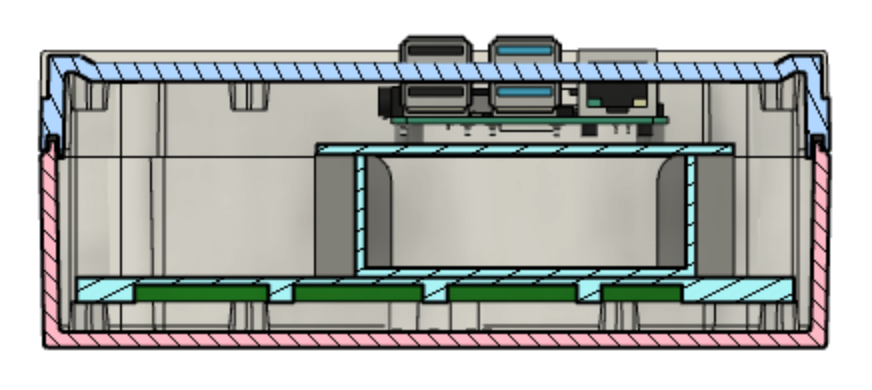
\includegraphics[scale=0.25]{Sections/Konstruktion_des_Aufbaus/Schnitt_Installationsbox_V_0.1}
	\end{center}
	\caption{Schnitt Installationsbox V 0.1}
	\label{fig:Schnitt_Installationsbox_V_0.1}
\end{figure}

Bei der Finalisierung des Aufbaus ist nochmals aufgefallen, wie maßungenau der 3D-Drucker arbeitet, so dass die Akkuwanne längs aufgesägt und die Löcher für die Schrauben aufgeweitet werden mussten.

\begin{figure}[h]
	\begin{center}
		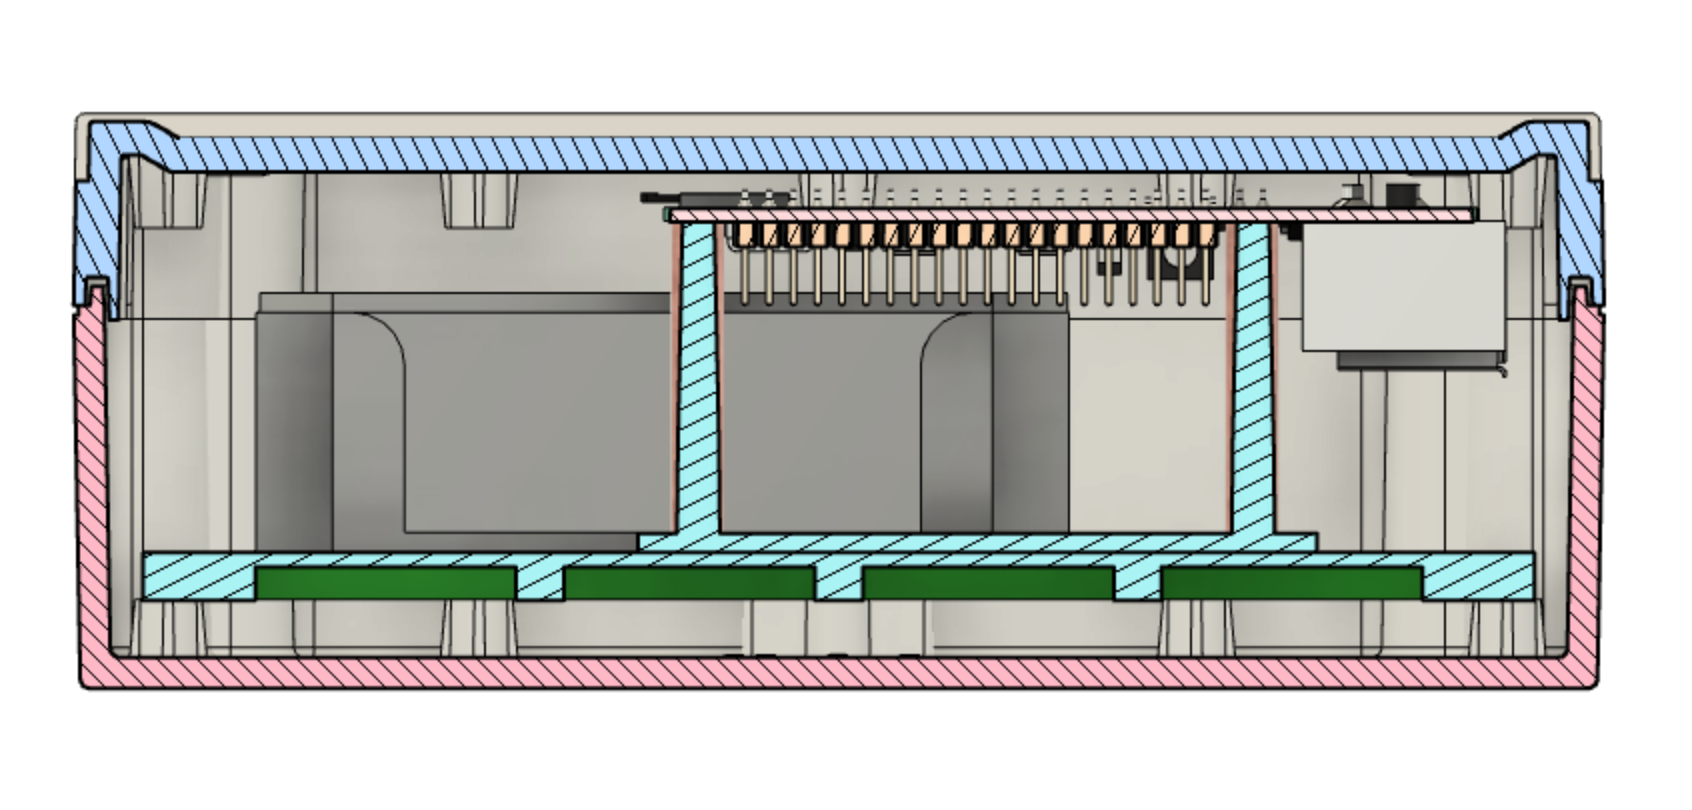
\includegraphics[scale=0.28]{Sections/Konstruktion_des_Aufbaus/Schnitt_Installationsbox_V_0.2}
	\end{center}
	\caption{Schnitt Installationsbox V 0.2}
	\label{fig:Schnitt_Installationsbox_V_0.2}
\end{figure}

\subsection{Positionierung der Baugruppen entlang eines Arrays}

Um die Mikrofone entlang einer Linie positionieren zu können, wurde ein vorhandenes Aluminiumprofil von itme aus der Serie 6 in den Dimensionen 1100 x 30 x 30 eingesetzt, auf welchem die Gehäuse der Mikrofone mit Nutensteinen in definierten Abständen montiert werden können. Dazu wurden am Mikrofongehäuse jeweils rechts und links zwei Befestigungspunkte für M4 Schrauben designt. Als Gegenstück werden wieder Nutensteine eingesetzt.

Das Profil an sich wird, wie oben beschrieben, auch mittels eines Nutensteins auf dem Stativ befestigt. Die Installationsbox wird ebenfalls mit Nutensteinen mittig am Profil befestigt.

\newpage